\section{Results}
\label{sec:results}

    The honeypot records both time stamps, and 
    interaction logs. Analysis of each will be handled separately 
    in subsections \ref{sec:time_analysis} and 
    \ref{sec:session_analysis}. 

    Then in section \ref{sec:irish_analysis} I take 
    a brief look at the origins of attacks.

\subsection{Statistical analysis of attack data}
\label{sec:time_analysis}

    The honeypot has been active since 12. of January
    2019, and until the 19. of March has logged 
    812013 individual SSH attacks. 


    The rate of attacks has been relatively constant over
    time (see figure \ref{fig:attacks_over_time}), with 
    the notable exception of the 12. of January and of 25. 
    January. The low amount of attacks on 12. of January is due 
    to how late I set the server up. 
    The dip in attack rate on the 25 is as of yet 
    unexplained.


    \begin{figure}[H]
        \centering
        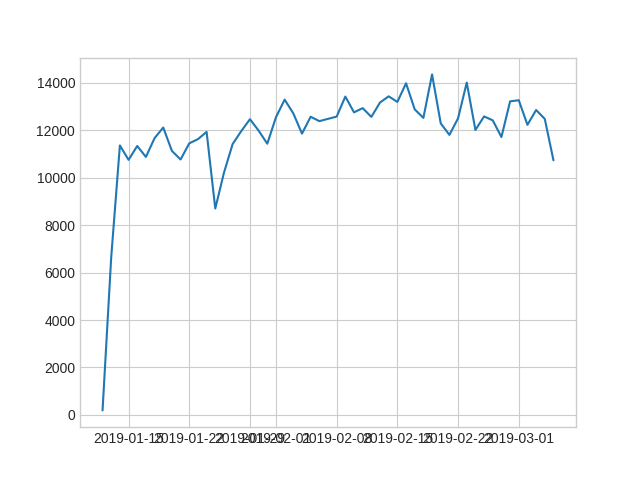
\includegraphics[width=0.85 \textwidth]{src/images/over_time.png}
        \caption{Rate of attacks from 12. Jan to 5. March}
        \label{fig:attacks_over_time}
    \end{figure}


    If the same done over the week (see figure \ref{fig:over_week}), 
    there is a seemingly
    non-random pattern that can be discerned, in that 
    over the weekend, the rate becomes more varied.


    \begin{figure}[H]
        \centering
        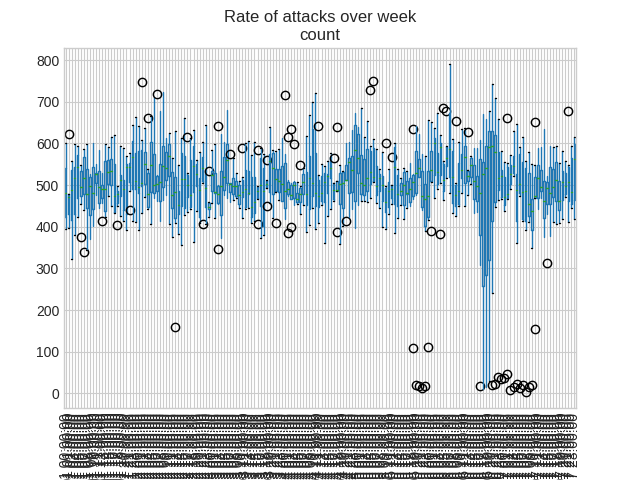
\includegraphics[width=0.8\textwidth]{src/images/week_unfiltered.png} 
        \caption{Rate of attacks plotted over a 'typical' week.}
        \label{fig:over_week}
    \end{figure}

    To preform the next two tests, I grouped the attacks by the
    date and time that they were launched, then grouped them 
    again by the time of day they were launched, taking the
    mean of the attack rates.

    To discover if there exists a relationship between the 
    time of day and attacks received, I attempted to use 
    autocorrelation as provided by the pandas library,
    but did not yield significant results. Either meaning that
    there is no correlation, or that the correlation is not 
    linear. 

    To discover if the mean attack rates over each hour of the
    day are likely to have been observations drawn from the same
    distributions, I preformed an 
    analysis of variance test (\textit{ANOVA}). 
    For this test I included all weekdays.

    This test resulted in a P value of 0.0395, which
    is enough to reject the hypothesis that the distributions
    of attacks over the hours of the day are equivalent (see table
    \ref{tab:anova_launches}).


    % df       sum_sq     mean_sq         F    PR(>F)
    % count       1.0   169.713862  169.713862  3.575061  0.060396
    % Residual  166.0  7880.286138   47.471603       NaN       NaN
    \begin{table}[H]
        \centering
        \begin{tabular}{|l|l|l|l|l|l|}
            \hline
                 & df    & sum\_sq     & mean\_sq   & F        & PR(\textgreater{}F) \\ \hline
        count    & 1.0   & 169.713862  & 169.713862 & 3.575061 & 0.060396            \\ \hline
        Residual & 166.0 & 7880.286138 & 47.471603  & NaN      & NaN \\\hline  
        \end{tabular}
        \caption{Anova Results for attack launch rate and time of day}
        \label{tab:anova_launches}
    \end{table}

    Graphing the rate of attacks launched suggests that 
    it is most popular for hackers to launch their attacks at
    around 05:00 in the morning (see figure \ref{fig:over_day})

    \begin{figure}[H]
        \centering
        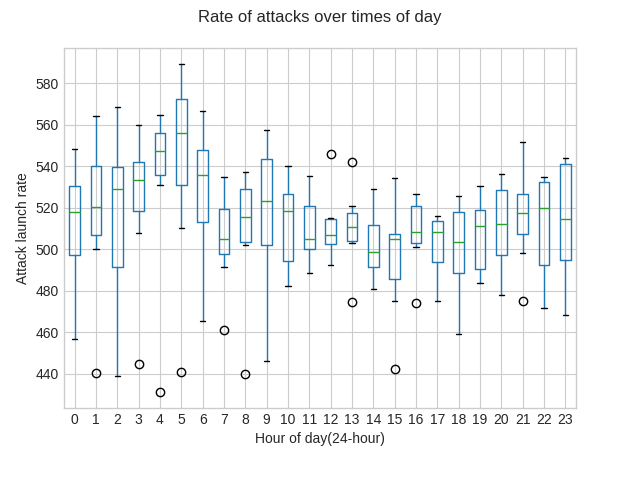
\includegraphics[width=0.85\textwidth]{src/images/rate_over_day.png}
        \caption{Anova results on testing rates of attacks launched over the time of day.}
        \label{fig:over_day}
    \end{figure}

    Repeating this test for the rates of attacks received, 
    does not yield a P value significant at the 0.05 level (see 
    table \ref{tab:anova_received}),
    however graphing it still shows the 05:00 peak. 
    
    \begin{table}[H]

        \centering
        \begin{tabular}{|l|l|l|l|l|l|}
        \hline
                 & df    & sum\_sq     & mean\_sq   & F        & PR(\textgreater{}F) \\ \hline
        count    & 1.0   & 169.713862  & 169.713862 & 3.575061 & 0.060396            \\ \hline
        Residual & 166.0 & 7880.286138 & 47.471603  & NaN      & NaN                 \\ \hline
        \end{tabular}
        \caption{Anova results on testing rates of attacks received over the time of day.}
        \label{tab:anova_received}
    \end{table}


    \begin{figure}[H]
        \centering
        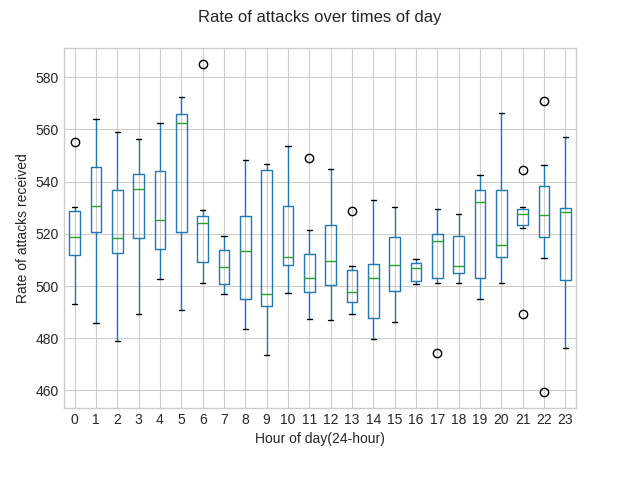
\includegraphics[width=0.85\textwidth]{src/images/rate_over_day_received.png}
        \caption{Rates of attacks received over the time of day.}
        \label{fig:over_day}
    \end{figure}

\subsection{Session log analysis}
\label{sec:session_analysis}

    The cowrie honeypot also captures the actions of 
    the attacker, as well as the files which he attempts
    to download and run on what he thinks is a compromised
    server. 


    One of the more intriguing factors that a number of the
    attack logs show, is an attempt to access a command
    called \texttt{'\\gisdfoewrsfdf'}. A command that 
    has I do not know what does, and a search yields no
    definitive results to what this command or script is. 

    Amongst the other things that are attempted, 
    are wiping the \texttt{./ssh/authorized\_keys} file and
    inserting a key, presumably of another infected
    device. 

    Twice during the period of 12. January to 1. March, 
    an attacker tried to download, and start an IRC bot.

    

\subsection{Origin of attacks}
\label{sec:origin_analysis}


    The most common countries of origin are Ireland, Russia,
    Germany, the Netherlands, and China.

    \begin{figure}[H]
        \centering
        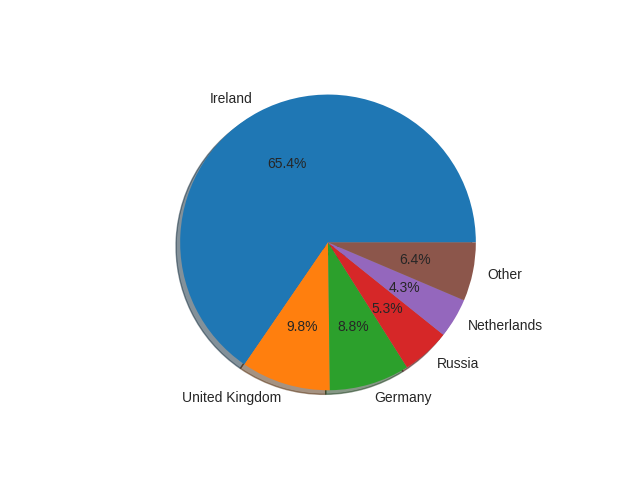
\includegraphics[width=0.8\textwidth]{src/images/countries_pie.png}
        \caption{Most common countries of origin.}
        \label{fig:country_pie}
    \end{figure}

    It was surprising how large the amount of attacks came from
    Ireland, and in fact upon closer inspection, 
    \texttt{'5.188.86.174'} is the originator of 
    $7.7\%$ of all attacks 
    (see figure \ref{fig:attacks_by_ip}).

    \begin{figure}[H]
        \centering
        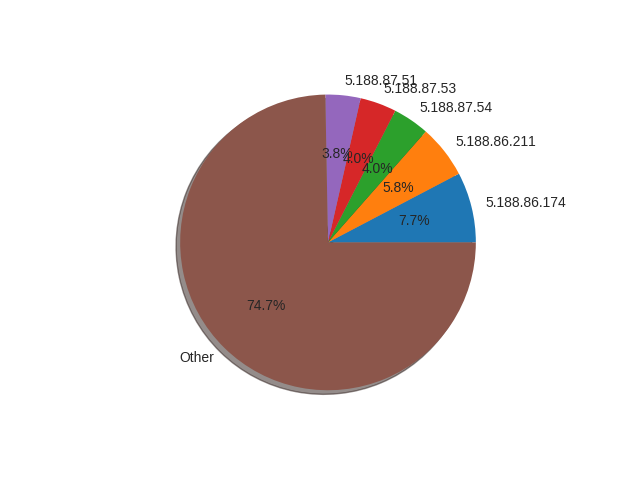
\includegraphics[width=0.8\textwidth]{src/images/ip_breakdown.png}
        \caption{Total attacks broken down by source address}
        \label{fig:attacks_by_ip}
    \end{figure}


    In fact, looking into the top offenders, 


    \texttt{'5.188.86.174'},
    \texttt{'5.188.86.211'},
    \texttt{'5.188.87.53'},
    \texttt{'5.188.87.54'}, and 
    \texttt{'5.188.87.55'} 

    reveals that all of them 
    are owned by \texttt{'Petersburg 
    Internet Network ltd.'}\abbrv{PIN}, a russian service provider 
    which has been implicated in both route-hijacking \cite{bogus_routing} 
    and allegedly with a gang of cyber criminals \cite{petersburg}

    
    A quick scan of the top offender, \texttt{'5.188.86.174'},
    preformed on the 19. of March revealed that it was a part of
    a TOR network. A secondary scan on the 4. of 
    April showed that the TOR ports were closed.

    This does not necessarily mean that all traffic from PIN
    registered IPs are russian in origin, but should be 
    subject for further inspection.